Ainda que poucas, as pesquisas sobre o uso de jogos digitais apontam sua efetividade como apoio educacional para as crianças e adolescentes (seção~\ref{sec:jogos_digiais_utilizacao}). Muito além da eficácia do jogo como ferramenta educacional, é preciso também observar a necessidade da inclusão da tecnologia na educação numa sociedade como a atual, onde o progresso tecnológico é constante e está presente no dia a dia da população.

No contexto das discussões acerca da inclusão do desenvolvimento do Pensamento Computacional na educação, em especial no Ensino Fundamental I, este trabalho apresenta uma proposta de jogo digital que está alinhado a este cenário. Para tanto, cada uma das fases do jogo tem como objetivo expor o jogador a uma situação que promova o desenvolvimento de algumas das habilidades citadas por Barr, V. e Stephenson~\cite{barr_bringing_2011} (seção~\ref{sec:habilidades}).

Neste capítulo, apresentamos uma proposta de jogo digital, “\textbf{As Aventuras de Ada e Turing}”. Para tanto, apresentamos o problema que incentivou a criação do jogo (seção~\ref{sec:problema}), em seguida, discorremos sobre a solução proposta (seção~\ref{sec:solucao}), expomos como foi feito o processo de implementação do jogo (seção~\ref{sec:implementacao}) e, finalmente, apresentamos a sua jogabilidade (seção~\ref{sec:jogabilidade}).

\section{Problema} \label{sec:problema}

Neste trabalho, vimos a forma como as \acrlong{TIC} podem ser utilizadas em sala de aula para auxiliar o processo de ensino e aprendizagem, a importância de uma abordagem diferenciada frente às necessidades tecnológicas dentro e fora da sala de aula, condição determinante para o desenvolvimento do Pensamento Computacional e, finalmente, algumas abordagens do uso de jogos como tecnologia auxiliar no processo de ensino e aprendizagem de diversos temas.

Apesar de encontrarmos alguns esforços no sentido de desenvolver o Pensamento Computacional no ambiente escolar, é visível que poucos desses trabalhos são direcionados ao Ensino Fundamental (seção~\ref{sec:jogos_desenvolvimento_pc}). Entretanto, a compreensão da tecnologia não é somente uma necessidade identificada na sociedade atual devido a sua presença no dia a dia, como também é assegurado pela Lei de Diretrizes e Bases da Educação Nacional n$^{\circ}$ 9.394~\cite{brasil_lei_1996}, na etapa do Ensino Fundamental, como um dos meios para a formação básica do cidadão.

Portanto, diante das necessidades expostas, identificamos uma questão: como apoiar o desenvolvimento do Pensamento Computacional no contexto escolar posto que o tema não é incluído no currículo? Destacamos alguns autores que defendem a utilização de jogos na educação para o desenvolvimento de habilidades (seção~\ref{sec:jogos_digiais_utilizacao}). No entanto, observamos uma escassez de jogos digitais educativos voltados ao desenvolvimento das habilidades do Pensamento Computacional (seção~\ref{sec:jogos_desenvolvimento_pc}). Além disso, grande parte dos autores encontrados durante a pesquisa apontaram o desenvolvimento do Pensamento Computacional como resultado direto do ato de programar. Desta forma, a grande maioria das propostas implantadas ou dos estudos apresentados pelos autores se preocupa em trazer os conceitos da Ciência da Computação (repetição, blocos, módulos, etc) para um jogo, tendo assim a programação como principal meio para o desenvolvimento do Pensamento Computacional.

Valente~\cite{valente_integracao_2016} destaca que outros países têm tentado criar condições para o desenvolvimento do Pensamento Computacional, buscando novas maneiras de trabalhar conceitos além de simplesmente aprender a programar. Também apresentamos autores como Yadav, Hong e Stephenson~\cite{yadav_computational_2016} e Wing~\cite{wing_computational_2006}, que defendem que a programação não é um aspecto essencial do Pensamento Computacional (seção~\ref{sec:definicao_pc}). Dadas as perspectivas, como trabalhar o desenvolvimento do Pensamento Computacional através de um jogo digital com foco no Ensino Fundamental I sem utilizar diretamente a programação como principal ferramenta do jogo?

\section{Solução} \label{sec:solucao}

Dentre os desafios de se propor uma solução para o desenvolvimento do Pensamento Computacional em ambiente escolar, a sua não inclusão no currículo da Educação Básica figura entre os maiores. Para contornar esse problema, nos baseamos no livro “\textit{Computer Science Unplugged}: Ensinando Ciência da Computação sem o uso do computador”~\cite{bell_computer_2011}. Nele, os autores propõem uma coletânea de atividades “desplugadas” para que qualquer pessoa aprenda conceitos da Ciência da Computação através de jogos e enigmas de vários tipos.

No site do livro\footnote{http://csunplugged.org/}, suas atividades são apontadas como introdutórias ao Pensamento Computacional através de conceitos da Ciência da Computação - números binários, algoritmos e compressão de dados -, além de destacar que a programação não é utilizada para tal. Nesse cenário, nos baseamos, para o desenvolvimento do jogo, na atividade 12, intitulada “Seguindo Instruções—Linguagens de Programação”~\cite[~p.101]{bell_computer_2011}. Nela, os autores apresentam o conceito “linguagem”, da Ciência da Computação, como um “vocabulário limitado de instruções que devem ser obedecidas” pelo computador. Essa habilidade, identificada pelos autores como dar e receber instruções, pode ser identificada como “usar o vocabulário”, presente na lista de habilidades do Pensamento Computacional. A partir disso, é proposta às crianças uma experiência sobre esse conceito da programação.

A atividade 12 foi escolhida por manifestar dois importantes aspectos relacionados ao desenvolvimento de um jogo digital para crianças no Ensino Fundamental I:

\begin{enumerate}
	\item ensinar conceitos de programação sem utilizar a programação em si;
	\item ter como público-alvo crianças a partir dos 7 anos de idade.
\end{enumerate}

A partir do conceito de dar e seguir instruções apontado pela atividade 12, foi necessário identificar as habilidades que queríamos desenvolver: usar o vocabulário; projetar soluções para problemas utilizando análise; projetar soluções para problemas utilizando análise e criação de algoritmo; e realizar testes e depuração~\cite{barr_bringing_2011}. Buscamos relacionar em maiores detalhes cada uma destas habilidades a fases específicas do protótipo desenvolvido (seção~\ref{ssec:dinamica}).

Tendo como base os fundamentos supracitados e relacionados ao Pensamento Computacional e tendo como inspiração dois personagens importantes da história da Computação - Ada Lovelance e Alan Turing - - criamos o protótipo do jogo, chamado “\textbf{As Aventuras de Ada e Turing}”. Buscamos, através dele, mostrar que é possível trabalhar algumas habilidades do Pensamento Computacional, utilizando o apelo lúdico do jogo, sem necessariamente exigir do aluno conhecimentos de programação.

\section{Implementação} \label{sec:implementacao}

A implementação de jogos digitais no cenário atual é possível através de diversas ferramentas. Para \textit{smartphones} que utilizam o sistema operacional Android, por exemplo, existe a possibilidade de usufruir do ambiente de desenvolvimento \textit{Android Studio}\footnote{https://developer.android.com/studio}, porém observadas as dificuldades de entrega em curto prazo, equipe de desenvolvimento pequena, necessidade de ferramentas gratuitas e portabilidade para o maior número de dispositivos possível, encontradas para o desenvolvimento de um jogo digital educativo, procuramos ferramentas que fossem mais adequadas a esse contexto.

\subsection{Ferramenta} \label{ssec:ferramenta}

Após a pesquisa por diversas ferramentas, optamos pelo \textit{framework} Corona SDK\footnote{Todos os tutoriais, kit de desenvolvimento e plugins para o Corona são disponibilizados diretamente no site https://coronalabs.com/}. Esta escolha deve-se ao fato de ele fornecer soluções para a maioria dos obstáculos para o desenvolvimento de um software educativo, entre eles:

\begin{itemize}
	\item desenvolvimento rápido: oferece uma série de tutoriais e ferramentas inclusas no próprio kit de desenvolvimento, a exemplo do simulador em tempo real para vários modelos de dispositivos, o que possibilita que a entrega seja feita em menos tempo. Além disso, o Corona serve como ferramenta para o desenvolvimento do protótipo e do produto final, isto é, o protótipo que desenvolvemos é funcional e pode ser utilizado diretamente no celular;
	\item gratuidade: o kit de desenvolvimento pode ser obtido de forma gratuita e, apesar de alguns \textit{plugins} serem pagos, é possível criar jogos e aplicativos completos sem custo;
	\item multiplataforma: através do kit de desenvolvimento do Corona é possível desenvolver apenas um código e disponibilizá-lo em várias plataformas (iPhone e iPad da Apple, \textit{smartphones} e \textit{tablets} Android, Amazon Fire, Mac Desktop, Windows Desktop, e até mesmo TVs conectadas com Apple TV, Fire TV, e Android TV), ampliando, assim, o público beneficiado e reduzindo o tempo de desenvolvimento.
\end{itemize}

O Corona é baseado em Lua, linguagem de \textit{script} amplamente utilizada para o desenvolvimento de jogos como Angry Birds \texttrademark e Civilization \texttrademark, permitindo, ainda, a importação de bibliotecas nativas ou \acrshort{API}. Portanto, consideramos esta uma ferramenta com curva de aprendizado curta, que permite a integração com outras ferramentas, além de já ser usada por programadores profissionais, escolas, e universidades para o desenvolvimento de jogos interativos, aplicativos educativos, entre outros.

Os cenários do jogo foram criados utilizando o editor de mapas \textit{Tiled}\footnote{Disponível para \textit{download} no site http://www.mapeditor.org/}. Com ele é possível criar todo o cenário, importando-o posteriormente para o Corona SDK. Além disso, o desenvolvimento do jogo “\textbf{As Aventuras de Ada e Turing}” exigiu a utilização das bibliotecas\footnote{As bibliotecas são conjuntos de códigos auxiliares independentes, que provém serviços para o programa principal.}:

\begin{itemize}
	\item GBCDataCabinet: \textit{plugin} de persistência usado para salvar e restaurar os jogos cadastrados.
	\item fms: máquina de estados finitos usada para sequenciar e controlar os eventos de cada fase, verificar ações do usuário e mostrar mensagens e animações.
	\item Ponytiled: usada em conjunto com o \textit{Tiled} para gerenciar todas as imagens, incluindo os locais onde devem ocorrer colisões\footnote{Eventos onde o personagem colide com elementos fixos do cenário (paredes, móveis, outros personagens, etc.}. 
\end{itemize}

Todas as bibliotecas são disponibilizadas gratuitamente e de fácil integração com o kit de desenvolvimento do Corona. A utilização delas foi responsável por reduzir o tempo de desenvolvimento do projeto, visto que a colisão dos personagens com áreas não andáveis do jogo, por exemplo, não precisou ser implementada do zero.

Além disso, as imagens empregadas no jogo foram retiradas dos \textit{sites} Kenney\footnote{http://kenney.nl/} e Freepik\footnote{https://br.freepik.com/}, sendo que elas podem ser usadas livremente em projetos, sejam eles comerciais ou não.

\section{Jogabilidade} \label{sec:jogabilidade}

O jogo “\textbf{As Aventuras de Ada e Turing}” foi elaborado a partir da proposta de criar algo que desenvolvesse habilidades do Pensamento Computacional e fosse atrativo para crianças. Porém, um dos elementos essenciais para o desenvolvimento de um jogo interessante depende de um enredo também interessante e que atraia a atenção do jogador para a história~\cite{arruda2014fundamentos}. A seguir, é detalhada a dinâmica do jogo através do enredo, dos primeiros desenhos e das principais cenas do jogo, além das justificativas quanto à forma como as habilidades que selecionamos do Pensamento Computacional foram trabalhadas em cada fase.

\subsection{Enredo} \label{ssec:enredo}

O público-alvo do jogo “\textbf{As Aventuras de Ada e Turing}” são crianças a partir de 7 anos. Com base nisso, o enredo foi pensado para contemplar parte do dia a dia de estudantes dessa faixa etária, passando pela Casa, Escola e Restaurante:

Hoje é mais um dia normal na vida de Ada, porém sua mãe a presenteia com uma bicicleta e um desafio: percorrer a cidade ajudando algumas pessoas e voltar para Casa no menor tempo possível para ganhar uma surpresa. Entretanto, seu irmão Turing ouviu a proposta da mãe e resolveu criar uma competição. Será que Ada conseguirá chegar em Casa antes de Turing? No caminho, ela terá que ajudar o professor a organizar a bagunça deixada pelos alunos na Escola e também ajudar o cozinheiro a preparar uma receita bem gostosa, isso tudo usando o que as pessoas a ensinam para chegar sempre na frente do irmão.

O nome do jogo, “\textbf{As Aventuras de Ada e Turing}”, foi inspirado em dois dos maiores nomes para o desenvolvimento da Ciência da Computação: Ada e Turing. A escolha dos nomes teve como intuito homenagear e aproximar o público-alvo de nomes que ajudaram a moldar a sociedade atual, na qual a tecnologia faz parte do dia a dia. Apesar do enredo ser contado com Ada como o personagem principal e Turing como o irmão coadjuvante, o jogo permite que os papéis sejam invertidos dependendo do personagem escolhido inicialmente pelo jogador.

\subsection{\textit{Mockups}} \label{ssec:mockups}

\textit{Mockups} são protótipos criados no início do projeto, são normalmente utilizados para adquirir \textit{feedback} sobre desenhos ou ideias logo no início do planejamento~\cite{interaction_design_foundation_mock-ups_nodate}. Assim, é possível visualizar os conceitos a serem implementados com baixo ou nenhum custo, visto que os \textit{mockups} podem ser elaborados em quadros, \textit{softwares}, ou mesmo em folhas de papel.

Para “\textbf{As Aventuras de Ada e Turing}”, concebemos os desenhos iniciais em folhas de papel com o objetivo de ver como ficariam dispostos os elementos na interface e quais imagens precisaríamos encontrar para a criação do jogo. As primeiras ideias foram desenvolvidas com todos os personagens sendo ratos, porém, a dificuldade de encontrar pessoas que confeccionassem os desenhos dos personagens fez com que adaptássemos o jogo para utilizar imagens de licença gratuita.

O protótipo jogável consiste em três fases, que se passam na Casa, Escola e Restaurante, de modo que esses três locais estão agrupados no Mapa da Cidade. O primeiro esboço (\refFig{fig:tutoriais}), ainda utilizando a ideia anterior de ratos, apresenta falas dos personagens. Entretanto, essa abordagem ocupava muito espaço de tela, fazendo com que a área de movimento dos personagens fosse reduzida. 

\figura[H]{tutoriais}{Primeiro \textit{mockup} das falas dos personagens}{fig:tutoriais}{width=0.8\textwidth}

A solução desse problema foi encontrada através do uso de balões de diálogo (\refFig{fig:dialogo}), versão final do protótipo. Essa abordagem de diálogo é muito utilizada por jogos de \acrshort{RPG}\footnote{\acrshort{RPG}, é uma sigla inglesa para \acrlong{RPG}, um “jogo de contar histórias”, onde os jogadores interpretam personagens dentro de uma história narrada por um “mestre”~\cite{cabalero_o_2007}.}, a exemplo do jogo Pokémon, usado no dispositivo \textit{Gameboy}. Dessa forma, é possível introduzir tutoriais com os personagens secundários conversando com o jogador, além de contextualizar o jogador na cena em que ele está.

\figura[H]{dialogo}{Interface que representa as falas dos personagens}{fig:dialogo}{width=0.6\textwidth}

As telas de Login e de Cadastro de novo jogador também foram esboçadas inicialmente e, por serem telas mais simples e com pouca interação com o usuário, se mantiveram quase idênticas à ideia original. Nos \textit{mockups} dessas interfaces (\refFig{fig:telas_iniciais}) era possível que o usuário escolhesse entre as opções \textbf{Novo Jogo} ou \textbf{Continuar} o jogo de onde parou, e a tela de Cadastrar um novo jogador, na qual o jogador deve informar o nome desejado e o personagem que deseja ser, para que o progresso do jogo seja salvo.

\figura[H]{telas_iniciais}{\textit{Mockups} das interfaces de \textit{Login} e Cadastro de novo jogador}{fig:telas_iniciais}{width=0.6\textwidth}

Cada uma das fases e o Mapa da Cidade também foram desenhados antes de serem implementados. Apesar de ser possível criar a prototipação das telas diretamente com o \textit{software} Tiled, fazer e modificar os desenhos demandava muito tempo, portanto criamos os desenhos em papel e só então o protótipo foi desenvolvido. Assim, foi possível projetar as telas considerando os movimentos que o personagem iria fazer para então criar o protótipo funcional (\refFigs{fig:mockup_fase_2}{fig:mockup_fase_3}).

\figura[H]{mockup_fase_2}{\textit{Mockup} da fase 2 do jogo “\textbf{As Aventuras de Ada e Turing}”}{fig:mockup_fase_2}{width=0.8\textwidth}

\figura[H]{mockup_fase_3}{\textit{Mockup} da fase 3 do jogo “\textbf{As Aventuras de Ada e Turing}”}{fig:mockup_fase_3}{width=0.8\textwidth}

Após a definição dos \textit{mockups}, o processo de implementação das telas foi realizado de forma ágil, uma vez que não foi necessário refazer as interfaces diversas vezes quando a ideia inicial se mostrava ineficaz ou apresentava erros de planejamento.

\subsection{Dinâmica} \label{ssec:dinamica}

Os \textit{mockups}, cenas e roteiro do jogo “\textbf{As Aventuras de Ada e Turing}” foram criados em paralelo. Isso se deve ao fato de estarem intimamente relacionados, visto que os diálogos interferem nas cenas e na apresentação do conjunto na tela. 

Para manter o controle da estrutura e sequência do jogo, foi criado um Documento de Design do Jogo (Apêndice~\ref{ap:design}). Conforme Pedersen~\cite{pedersen2009game}, esse documento é uma ferramenta textual criada para descrever todas as características de um jogo: informações básicas de premissa, conceitos, personagens e cenários, além de poder incluir detalhes como sons e níveis. No caso do presente projeto, a criação do referido documento foi essencial para manter as duas autoras alinhadas ao mesmo objetivo.

O projeto do jogo “\textbf{As Aventuras de Ada e Turing}”, descrito no Documento de Design (Apêndice~\ref{ap:design}), é composto por quatro cenas: a Casa do personagem principal (\refFig{fig:casa}), a Escola (\refFig{fig:escola}), o Restaurante (\refFig{fig:restaurante}) e o Mapa (\refFig{fig:mapa}), de forma que este último agrega todos os locais anteriores.

O Mapa (\refFig{fig:mapa}), representa uma cena de transição e funciona como tela de controle do progresso do jogador.

\figura[H]{casa}{Interface que representa a cena da Casa de Ada e Turing}{fig:casa}{width=0.6\textwidth}

\figura[H]{escola}{Interface que representa a cena da Escola}{fig:escola}{width=0.6\textwidth}

\figura[H]{restaurante}{Interface que representa a cena do Restaurante}{fig:restaurante}{width=0.6\textwidth}

\figura[H]{mapa}{Interface que representa a cena do Mapa}{fig:mapa}{width=0.6\textwidth}

Cada elemento do jogo “\textbf{As Aventuras de Ada e Turing}” foi planejado com o intuito de estimular o jogador e desenvolver habilidades do Pensamento Computacional sem perder o aspecto lúdico de um jogo. O protótipo do jogo envolve três fases, de forma que quatro das dez habilidades listadas por Barr, V. e Stephenson~\cite{barr_bringing_2011} foram utilizadas:

\begin{itemize}
	\item Usar o vocabulário.
	\item Projetar soluções para problemas utilizando análise.
	\item Projetar soluções para problemas utilizando análise e criação de algoritmo.
	\item Realizar testes e depuração.
\end{itemize}

A seguir, percorremos todo o fluxo do jogo apresentando os elementos que compõem “\textbf{As Aventuras de Ada e Turing}”, além dos objetivos que constituíram cada um deles.

\subsubsection{Cadastro de Novo Jogador} \label{sssec:cadastro}

O jogo inicia com duas possibilidades exibidas pelo Menu Inicial (\refFig{fig:menu_inicial}). Nele, o jogador pode iniciar um Novo Jogo ou Continuar um jogo que ele já havia começado. Caso inicie um Novo Jogo, o jogador deverá fazer um Novo Cadastro (Figuras~\ref{fig:cadastro}) informando o personagem que deseja ser: Ada ou Turing (Figura~\ref{fig:cadastro_personagens}) e o nome para o cadastro do Novo Jogo (Figura~\ref{fig:cadastro_nome}). A partir do momento que o jogador escolhe um personagem, automaticamente o outro se torna o personagem secundário que irá acompanhá-lo por todo o percurso do jogo. Caso o jogador escolha Continuar o Jogo, a interface de jogos salvos (\refFig{fig:save}) exibe os cadastros salvos e o jogador poderá continuar de onde parou.

\figura[H]{menu_inicial}{Interface que representa o menu inicial}{fig:menu_inicial}{width=0.6\textwidth}

\begin{figure}[H]
\centering
\subfloat[Interface que representa a escolha do personagem]{
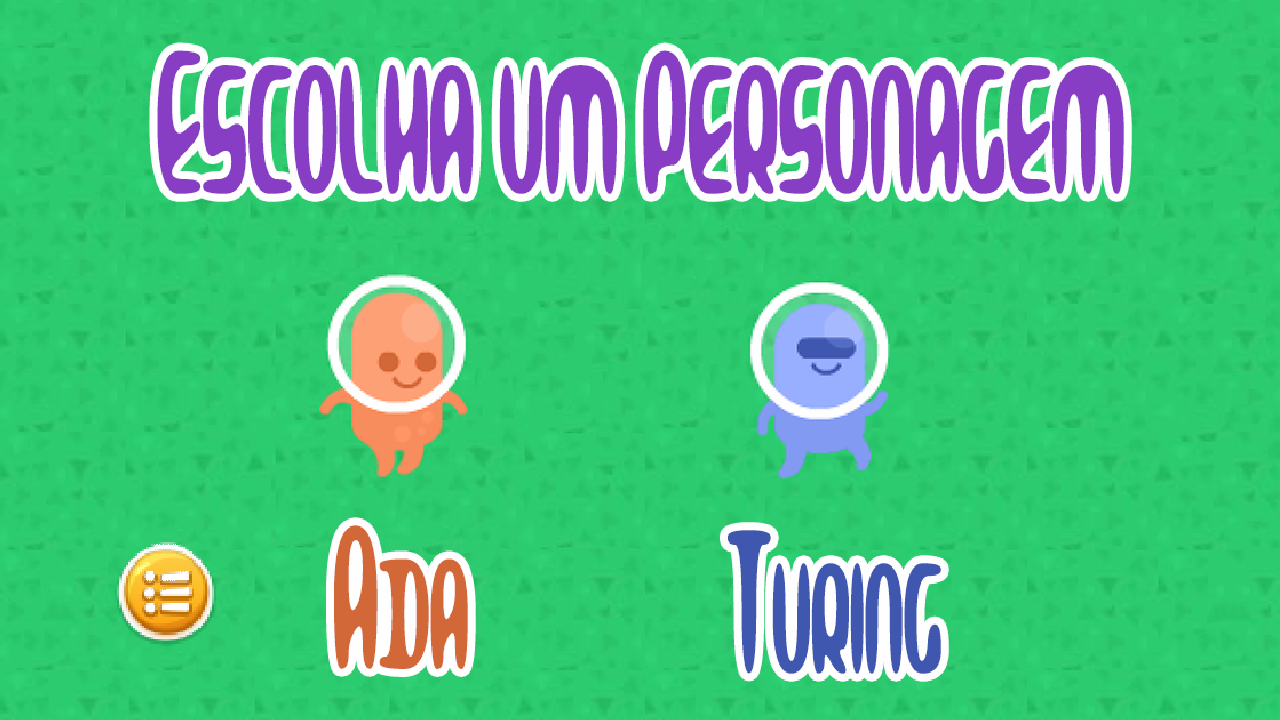
\includegraphics[height=3cm]{cadastro_personagens}
\label{fig:cadastro_personagens}
}
\quad %espaco separador
\subfloat[Interface que representa a minibiografia da Ada]{
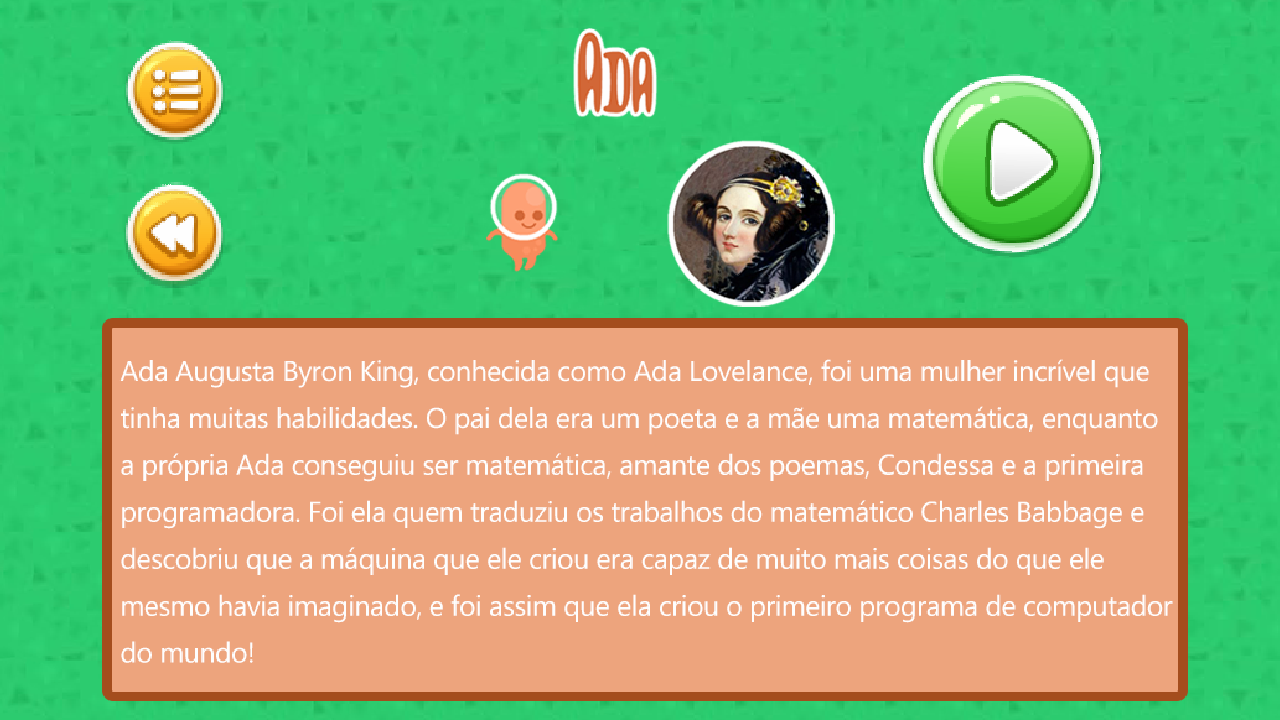
\includegraphics[height=3cm]{cadastro_descricao_ada}
\label{fig:cadastro_ada}
}
\quad %espaco separador
\subfloat[Interface que representa a minibiografia do Turing]{
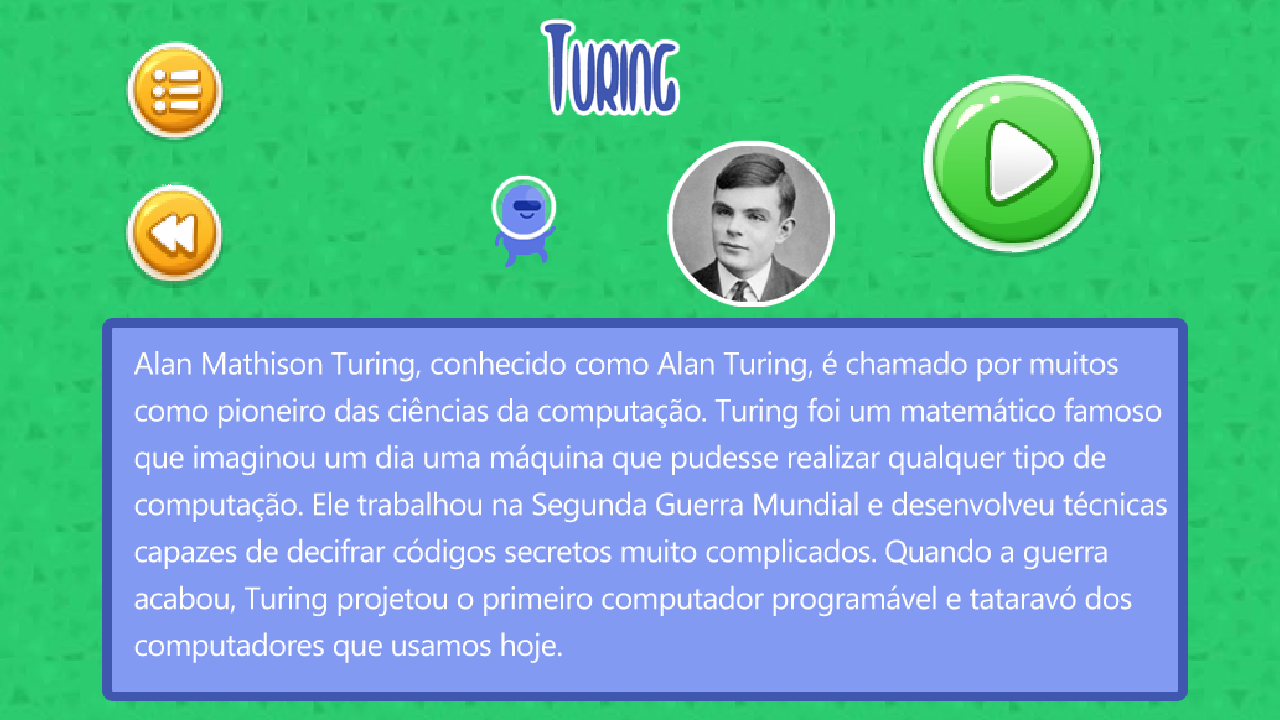
\includegraphics[height=3cm]{cadastro_descricao_turing}
\label{fig:cadastro_turing}
}
\quad %espaco separador
\subfloat[Interface que representa a inserção do nome]{
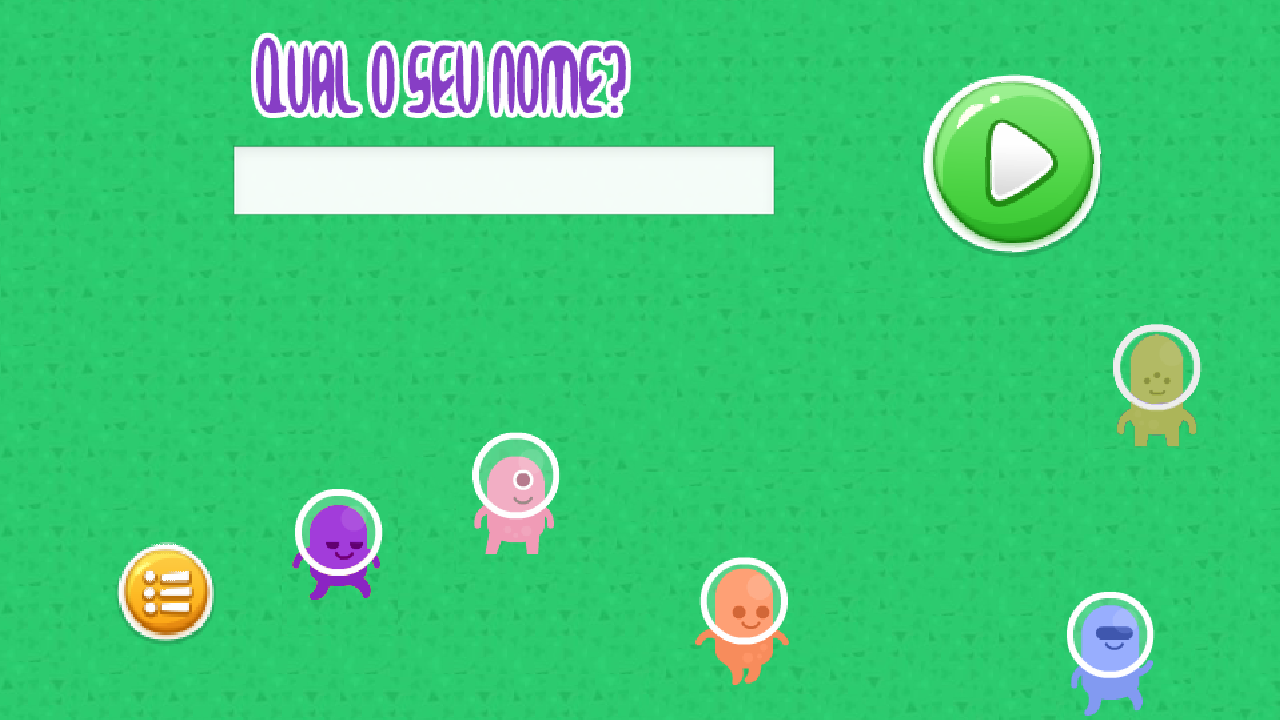
\includegraphics[height=3cm]{cadastro_nome}
\label{fig:cadastro_nome}
}
\caption{Interface que representa as etapas do cadastro}
\label{fig:cadastro}
\end{figure}

\figura[H]{save}{Interface que representa os cadastros salvos}{fig:save}{width=0.6\textwidth}

Ainda no Cadastro, é exibida uma minibiografia histórica dos personagens do jogo (Figuras~\ref{fig:cadastro_ada} e Figura~\ref{fig:cadastro_turing}), visto que Ada e Turing são dois nomes importantes para a Ciência da Computação e estão sendo homenageados no jogo. O texto das minibiografias (Tabela~\ref{tab:minibiografias}), criado pelas autoras, busca contar a história dos dois personagens utilizando uma linguagem adequada ao público-alvo e, dessa forma, aproximar o jogador de nomes que ajudaram a moldar a sociedade atual.

\begin{table}[H]
\centering
\caption{Minibiografias de Ada e Turing}
\label{tab:minibiografias}
\begin{tabular}{|l|p{12cm}|}
\hline
\textbf{Personagem} & \textbf{Minibiografia}                                                                                                                                                                                                                                                                                                                                                                                                                                                                                                \\ \hline
Ada                 & Ada Augusta Byron King, conhecida como Ada Lovelance, foi uma mulher incrível que tinha muitas habilidades. O pai dela era um poeta e a mãe uma matemática, enquanto a própria Ada conseguiu ser matemática, amante dos poemas, Condessa e a primeira programadora. Foi ela quem traduziu os trabalhos do matemático Charles Babbage e descobriu que a máquina que ele criou era capaz de muito mais coisas do que ele mesmo havia imaginado, e foi assim que ela criou o primeiro programa de computador do mundo! \\ \hline
Turing              & Alan Mathison Turing, conhecido como Alan Turing, é chamado por muitos como pioneiro das ciências da computação. Turing foi um matemático famoso que imaginou um dia uma máquina que pudesse realizar qualquer tipo de computação. Ele trabalhou na Segunda Guerra Mundial e desenvolveu técnicas capazes de decifrar códigos secretos muito complicados. Quando a guerra acabou, Turing projetou o primeiro computador programável e tataravó dos computadores que usamos hoje.                                    \\ \hline
\end{tabular}
\end{table}

\subsubsection{Fase 1: Casa} \label{sssec:fase_1}

Passadas as etapas de criação (ou seleção), o jogo em si começa na Casa (\refFig{fig:fase_1_1}). Nesta fase, o objetivo é desenvolver a habilidade de \textbf{usar o vocabulário}. Para tanto, o jogador passará por um treino interativo - expondo as instruções de direção e o conceito de repetição representado por uma bicicleta - onde a mãe irá instruí-lo sobre como os comandos do jogo funcionam enquanto uma animação destaca os elementos que devem ser utilizados (\refFig{fig:fase_1_2}). 

\figura[H]{fase_1_1}{Interface que representa a fase 1 do jogo “\textbf{As Aventuras de Ada e Turing}”}{fig:fase_1_1}{width=0.6\textwidth}

\figura[H]{fase_1_2}{Interface que representa a fase 1 do jogo “\textbf{As Aventuras de Ada e Turing}”}{fig:fase_1_2}{width=0.6\textwidth}

Os comandos e a dinâmica apresentados nas fases 1 e 2 (seção~\ref{sssec:fase_2}) estarão presentes em todas as outras fases. Desenvolvemos um treinamento mais lúdico, onde o usuário tem um objetivo e, através das instruções do personagem orientador da fase, realizará as ações de forma a aprender ativamente como os comandos funcionam.

É também nesta fase que o jogador é apresentado ao seu antagonista (\refFig{fig:fase_1_3}). Através dele pretendemos criar um elemento de competitividade, onde o jogador deve sempre tentar ultrapassar adversário.

\figura[H]{fase_1_3}{Interface que representa a primeira fase do jogo “\textbf{As Aventuras de Ada e Turing}”: apresentação do irmão/irmã}{fig:fase_1_3}{width=0.6\textwidth}

Ao finalizar a primeira fase, o jogo apresentará a primeira tela de \textit{feedback} (Figuras \ref{fig:feedbacks}), essa ação será repetida ao final de cada uma das fases. São três níveis de \textit{feedback}: 

\begin{enumerate}
	\item nenhuma estrela (Figura~\ref{fig:feedback_0}): o jogador não alcançou o objetivo da fase;
	\item uma estrela (Figura~\ref{fig:feedback_1}): o jogador completou o objetivo, porém não utilizou a habilidade do Pensamento Computacional desenvolvida na fase;
	\item duas estrelas (Figura~\ref{fig:feedback_2}): o jogador completou o objetivo, porém não utilizou a habilidade do Pensamento Computacional desenvolvida na fase tanto quanto poderia;
	\item três estrelas (Figura~\ref{fig:feedback_3}): o jogador completou o objetivo da fase e utilizou a habilidade do Pensamento Computacional desenvolvida na fase de forma adequada.
\end{enumerate}

\begin{figure}[H]
\centering
\subfloat[Nenhuma estrela]{
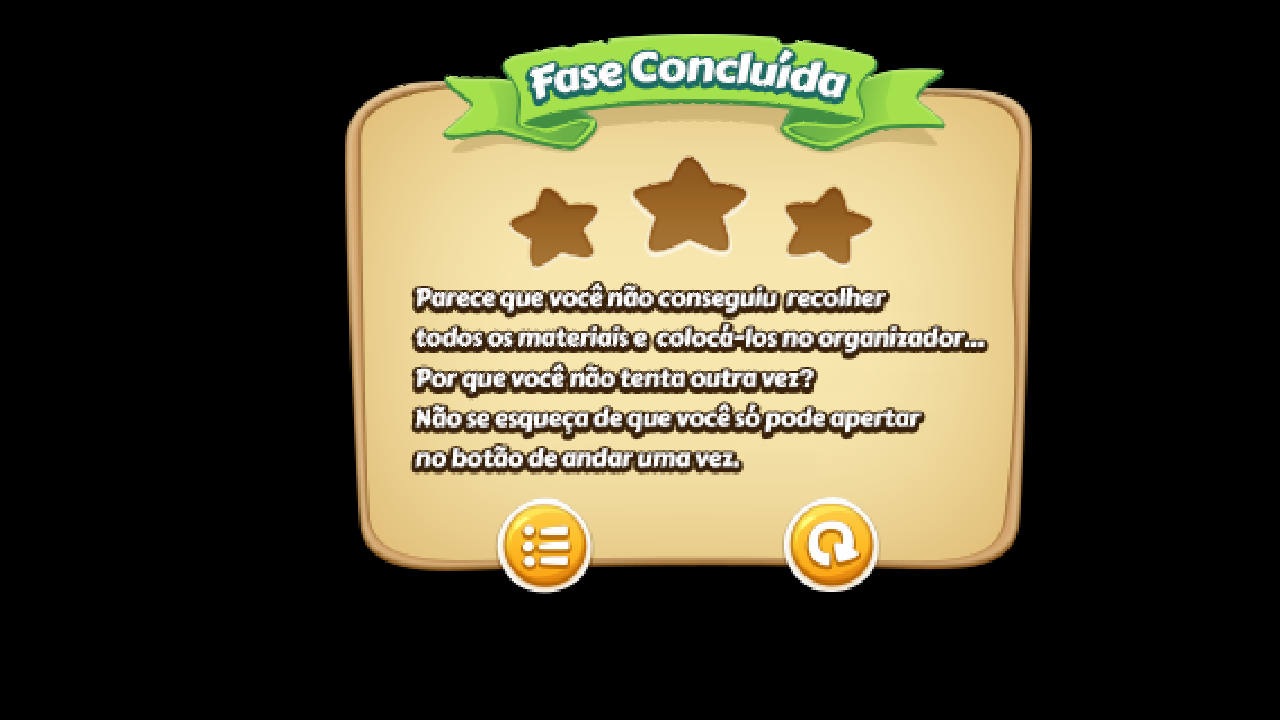
\includegraphics[height=3cm]{feedback_0}
\label{fig:feedback_0}
}
\quad %espaco separador
\subfloat[Uma estrela]{
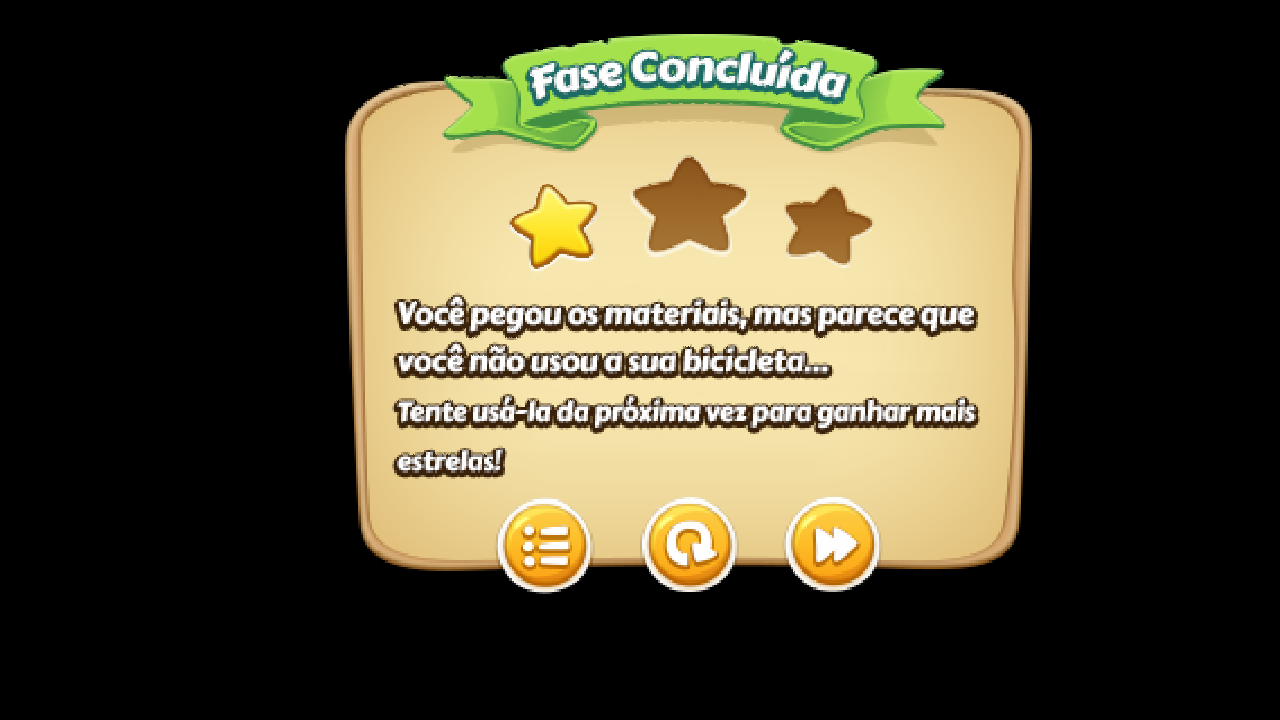
\includegraphics[height=3cm]{feedback_1}
\label{fig:feedback_1}
}
\quad %espaco separador
\subfloat[Duas estrelas]{
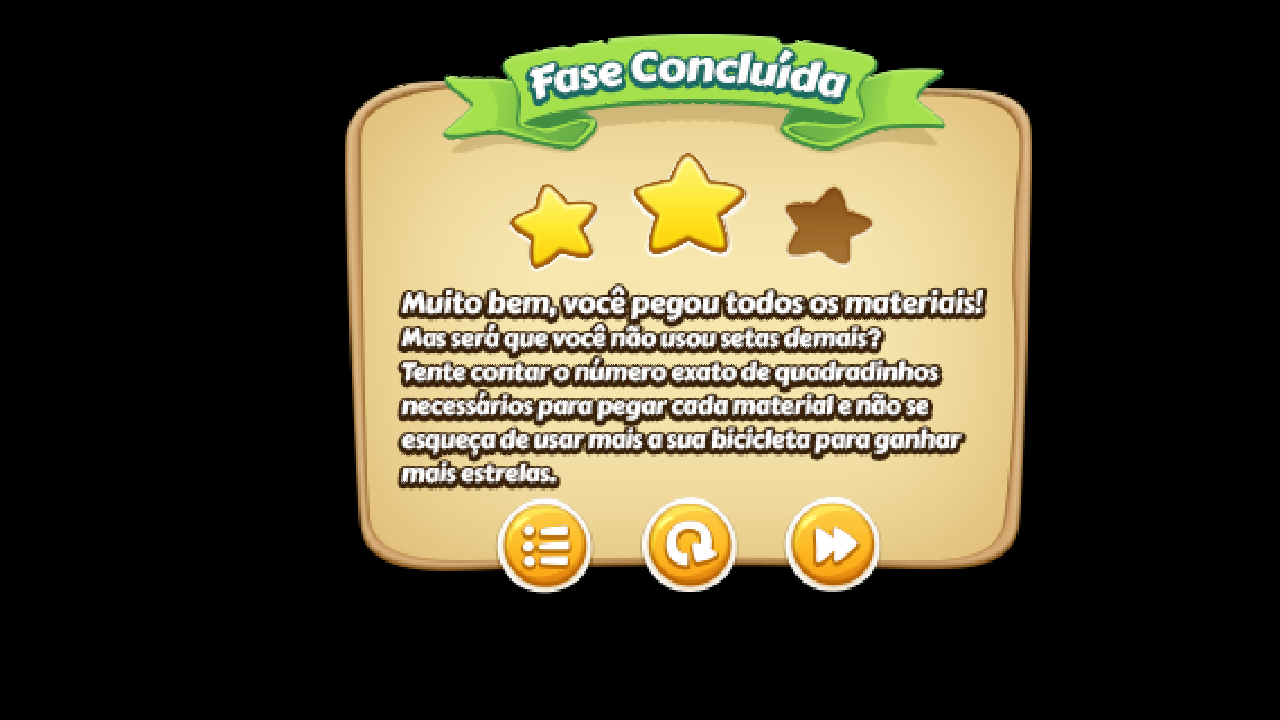
\includegraphics[height=3cm]{feedback_2}
\label{fig:feedback_2}
}
\quad %espaco separador
\subfloat[Três estrelas]{
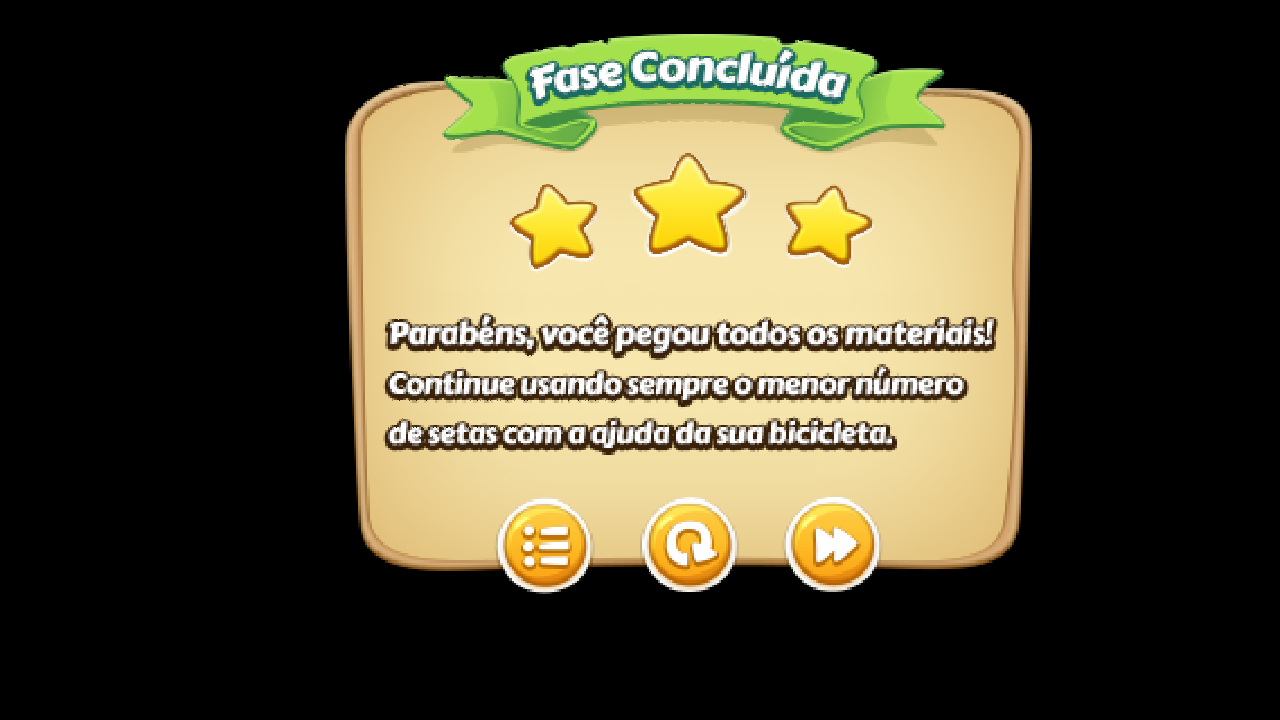
\includegraphics[height=3cm]{feedback_3}
\label{fig:feedback_3}
}
\caption{Telas de \textit{feedback}}
\label{fig:feedbacks}
\end{figure}

É preciso que os jogadores sejam capazes de aprender com os próprios erros, revendo e analisando seus passos, para que seja possível traçar uma nova estratégia em caso de fracasso, ou simplesmente para compreender por que obteve sucesso~\cite{paula_jogos_2016}. Desse modo, mais uma habilidade do Pensamento Computacional é incluída ao jogo: \textbf{realizar testes e depuração}, pois o jogador pode ver que poderia ter se saído melhor naquela fase e de que forma poderia melhorar, tendo a opção de jogar a mesma fase novamente para tentar obter um desempenho melhor.

Ainda trabalhando a habilidade de realizar testes e depuração, a movimentação do jogador é destacada à medida que o personagem se desloca (\refFig{fig:rastro}). Dessa forma é possível que ele reveja os pontos onde acertou ou errou.

\figura[H]{rastro}{Interface que representa o rastro do percurso feito pelo jogador}{fig:rastro}{width=0.6\textwidth}

Outro recurso utilizado pelo jogo é o Mapa (\refFig{fig:mapa}). Nele, o jogador continua treinando os comandos que aprendeu, posto que a movimentação nele segue a mesma dinâmica de todo o jogo. O Mapa também é utilizado para que o jogador tenha acesso a todas as fases, cada uma delas representada por uma construção, de maneira que as fases já concluídas são marcadas pelo número de estrelas recebidas e as fases que ainda não foram concluídas mostram as estrelas inativas (\refFig{fig:mapa_1}).

\figura[H]{mapa_1}{Interface que representa o Mapa com duas fases concluidas}{fig:mapa_1}{width=0.6\textwidth}

A partir da fase 2, o irmão ou irmã chegará na fase seguinte antes ou depois do jogador, dependendo de como for o seu desempenho no caminho realizado no mapa entre uma fase e outra. Nesses caminhos, o jogador terá uma quantidade limitada de repetições, e caso consiga chegar ao próximo destino, isto é, fase, usando a menor quantidade possível de instruções,  conseguirá chegar antes do irmão. Caso o jogador consiga realizar o caminho entre duas fases com a menor quantidade possível de instruções e, consequentemente, chegar antes do irmão, pelo menos duas vezes durante o jogo inteiro, a surpresa final ficará com o jogador. 

\subsubsection{Fase 2: Escola} \label{sssec:fase_2}

A fase 2 se passa na Escola (\refFig{fig:escola_1}) e continua utilizando os conceitos demonstrados na fase 1 (seção~\ref{sssec:fase_1}), porém limita as ações do jogador. Na fase 1, o jogador pode cumprir o objetivo em quantas etapas desejar. No entanto, nesta fase, ele deverá completar o objetivo utilizando um único conjunto de instruções, porém na ordem mais adequada, isto é, elaborar a melhor estratégia para pegar todos os materiais espalhados pela sala e depositá-los no organizador utilizando um único conjunto de instruções. Assim, pretendemos que o jogador \textbf{projete soluções para problemas utilizando análise}, mais uma habilidade do Pensamento Computacional.

\figura[H]{escola_1}{Interface que representa a fase 2 com os objetos espalhados pela sala de aula}{fig:escola_1}{width=0.6\textwidth}

\subsubsection{Fase 3: Restaurante} \label{sssec:fase_3}

A fase 3, por sua vez, foi desenvolvida para que o jogador \textbf{projete soluções para problemas utilizando análise e criação de algoritmo}. Com o intuito de desenvolver essa habilidade do Pensamento Computacional, o jogo propõe que o jogador complete uma receita em duas etapas. Para tanto, ele deve coletar os ingredientes espalhados pelo Restaurante de forma ordenada - obedecendo uma lista - e retornar cada uma das vezes com um conjunto de ingredientes ao cozinheiro. Novamente, o jogador estará utilizando todos os conceitos que aprendeu anteriormente, porém deverá seguir a ordem definida pelo cozinheiro. No Restaurante (\refFig{fig:restaurante_1}) é possível observar os ingredientes espalhados e a ordem em que a primeira lista deve ser entregue ao cozinheiro.

\figura[H]{restaurante_1}{Interface que representa a fase 3 com os objetos espalhados pelo Restaurante}{fig:restaurante_1}{width=0.6\textwidth}

O jogo “\textbf{As Aventuras de Ada e Turing}” chega ao fim quando o jogador retorna para Casa após ajudar todas as pessoas da cidade. Nesse momento, caso tenha conseguido chegar antes do irmão em pelo menos três fases, o jogador receberá a surpresa que foi prometida pela mãe. Caso contrário, perderá a aposta com o irmão e ficará sem a surpresa. No entanto, o jogo permite que o jogador refaça todas as fases para tentar conseguir a surpresa também. 
